% lualatex tenuki29
\nonstopmode


\documentclass[a4paper]{ltjsarticle}
\usepackage{listings}
\usepackage{graphicx}
\usepackage{here}
\title{手抜きについて}
\author{手抜きチーム}
\date{2019年3月25日}


\begin{document}

\maketitle

手抜きはCSAプロトコルで対局を行うコンピュータ将棋プログラムです。作者らが将棋のプログラムの仕組みを理解することを目的として開発しています。
リポジトリ:https://github.com/hikaen2/tenuki-d



\section{作者の紹介}

\subsubsection*{鈴木太朗}
鈴木はプログラマです。会社員をしています。
仕事のかたわら趣味の自転車と合唱に打ち込んでいます。
そのかたわら手抜きを作っていますが完成させる自信がありません
(夏休みの宿題を9月1日にやるタイプです)。
棋力は30級程度です。
Twitter: @hikaen2

\subsubsection*{玉川直樹}
玉川はP兼召喚士です。KPPとレーティングシステムを疑っています。将棋ウォーズ2段。
手抜きの定跡を手入力で作りました。
Twitter: @Neakih\_kick


\section{目標}

\subsection{今年の目標}

\begin{itemize}
\item 探索をマルチスレッドにする
\end{itemize}

Ryzenを買っちゃったのでマルチスレッドにします。
これからLazy SMPを実装します。
スレッドがよくわかりません。
実装できても正しく実装できているか分からない予感がします。

\begin{itemize}
\item KPPTで評価する
\end{itemize}

去年はなのはさんの評価バイナリでKP + PPで評価しました。
今年はAperyの評価バイナリ(大樹の枝形式)でKPPTで評価しようと思います。
Aperyの選定理由は評価バイナリがKPPTだからです。
予想として,静的評価に手番が含まれると静止探索がいらないか,もしくは軽くていいのではないかと思っています。

評価バイナリの自作については来年挑戦します。


\subsection{来年の目標}

\begin{itemize}
\item 評価バイナリを自作する
\end{itemize}


\subsection{去年までの目標と結果}

第28回世界コンピュータ将棋選手権:
\begin{itemize}
\item ルール通りに指す → 結果:ルール通り指した(けど千日手のチェックをしてない)
\item 投了する(第27回では王手放置していた) → 結果:投了した。一次予選4勝4敗
\item KPで評価する → 結果:なのはさんの評価バイナリでKP + PPで評価した
\end{itemize}

第27回世界コンピュータ将棋選手権:
\begin{itemize}
\item 出場する → 結果:出場した
\item 対局する → 結果:対局した。一次予選2勝5敗
\end{itemize}



\section{プログラムの構造}

この章では手抜きの構造の説明をします。

\subsection{データ構造}

盤面に81要素の1次元配列を使用しています。そのアドレッシングはこうです:

\begin{figure}[H]
  \centering
  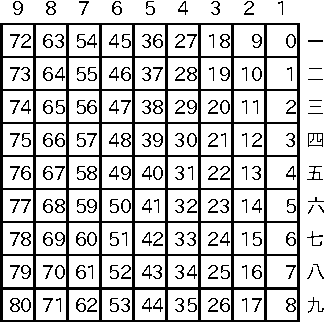
\includegraphics{fig/fig1.pdf}
  \caption{盤面のデータ構造}
\end{figure}

第28回世界コンピュータ将棋選手権では「壁」がありましたが,なくしました。
壁がないと,壁のレイアウトを考えなくて済む,盤面がコンパクトになる,zobrist hash seedもコンパクトになる,静的評価が簡単になる(盤面のアドレッシングと評価バイナリのアドレッシングが合っていれば)といった利点があります。
一方で合法手生成が複雑になる欠点があります(1段目と9段目が繋がっているので油断すると駒がワープする)。

盤面の各要素は0から28までの値を取ります。値の意味はこうです(次表のA列):

\begin{table}[H]
  \centering
  \caption{値の意味}
  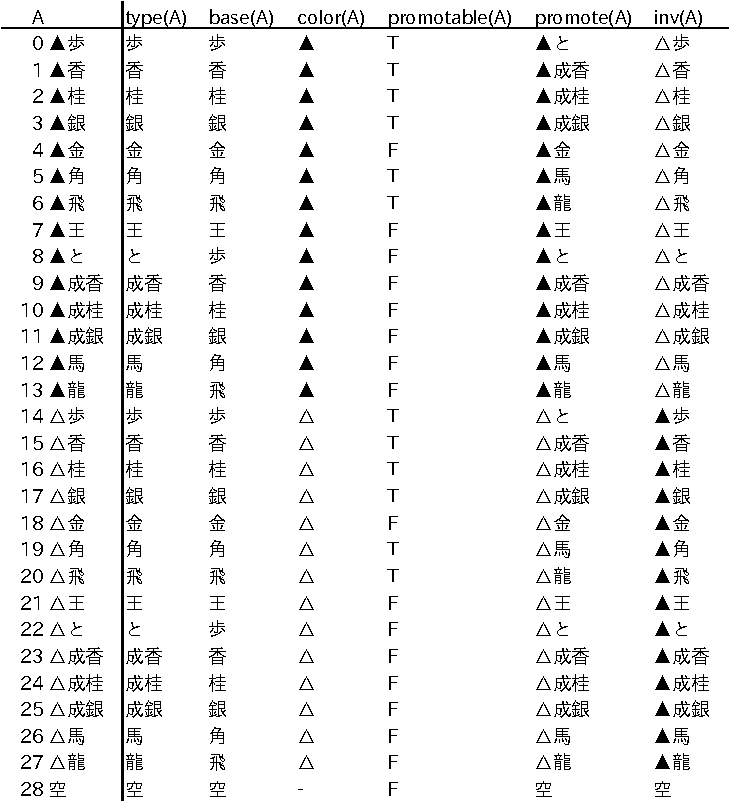
\includegraphics{fig/fig2.pdf}
\end{table}

第28回世界コンピュータ将棋選手権では手番と成りをビット演算で管理していましたが,表で管理するようにしました。
表で管理するとビットレイアウトを考えなくて済む利点があります。
一方,表を引くのに(ビット演算よりは)時間がかかる欠点がありそうです。

表のtype(A)の列からinv(A)の列まではA列の関数です。
意味はこうです:

\begin{itemize}
  \item type(A): Aから手番を除いた値を返す。
  \item base(A): Aから手番を除いて成りを戻した値を返す。駒を取ったときに使う。
  \item color(A): Aの手番を返す。
  \item promotable(A): Aが成れる駒かどうかを返す。
  \item promote(A): Aが成った駒を返す。
  \item inv(A): Aの手番を反転した駒を返す。
\end{itemize}

こうして見ると全部で6つあって多いように思います。
全部で4つくらいになってもいいような気がします。


\subsection{探索}

mini-max探索をしています。

\begin{itemize}
  \item αβ枝刈りをしています。最近やっとαβ枝刈りが何なのか分かるようになりました。
  \item null-move枝刈りをしています。
  \item 静止探索しています。
  \item 指し手だけの置換表(指し手表?)があります。表のエントリは指し手だけです。
  一般的な置換表のエントリにはミスヒット検出のために局面のハッシュ値が入れてありますが,手抜きでは入れていません。
  指し手だけの表なのでミスヒットしても害がないと考えているためです。しかしLazy SMPしはじめると問題があるかもしれません。
  \item Lazy SMPしたいです。
  \item futility枝刈りしていません。静的評価が差分評価でないからです。
\end{itemize}


\subsection{静的評価}

Apery, commit 3221627(2016年11月3日)の評価バイナリを使ってKPPTで評価する予定です。

\end{document}
